\begin{figure}[!t]
    \centering
    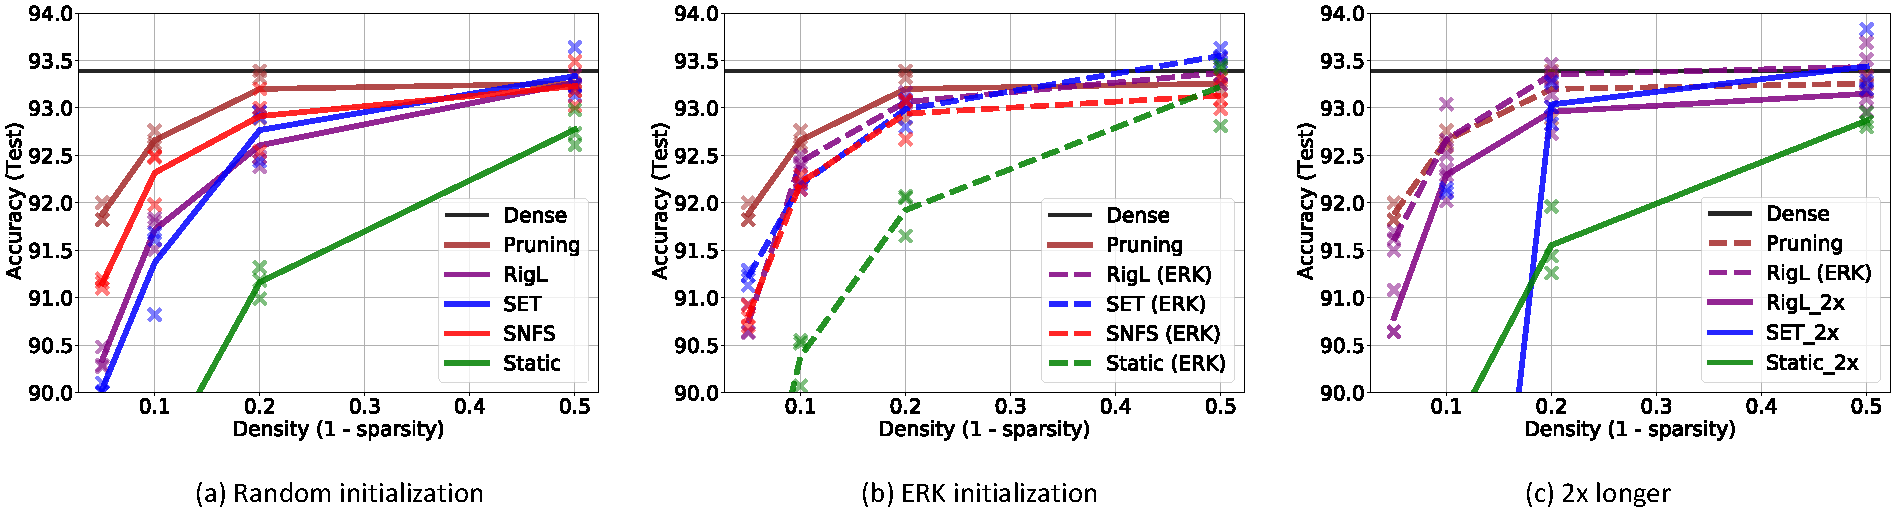
\includegraphics[width=1\textwidth]{../openreview/figs/cifar10_main.pdf}
    \captionsetup{aboveskip=\figureaboveskip,belowskip=\figurebelowskip}
    \caption{\textbf{Test Accuracy vs Sparsity on CIFAR-10,} plotted for Random initialization \textbf{(left)}, ERK initialization \textbf{(center)}, and for training $2\times$ longer \textbf{(right)}. Owing to random growth, SET can be unstable when training for longer durations with higher sparsities. Overall, \textit{RigL}\textsubscript{$2 \times$} (ERK) achieves highest test accuracy.}
    \label{fig:cifar10-main-results}
\end{figure}